% ============================================================================
%  Bohrin on 20 Public LeRobot Datasets
%  Compiles on Overleaf as-is (pdfLaTeX). No custom classes, no shell-escape,
%  no external downloads. Locally: `tectonic bohrin-benchmark.tex`
%  or `pdflatex bohrin-benchmark.tex` (run twice for cross-references).
% ============================================================================
\documentclass[10pt,a4paper]{article}

\usepackage[T1]{fontenc}
\usepackage[utf8]{inputenc}
\usepackage{lmodern}
\usepackage[margin=1in]{geometry}
\usepackage{graphicx}
\usepackage{booktabs}
\usepackage{caption}
\usepackage{xcolor}
\usepackage{amsmath}
\usepackage{microtype}
\usepackage[hidelinks]{hyperref}
% Let long typewriter paths wrap at separators instead of running off the margin.
\usepackage{url}
\urlstyle{tt}
\def\UrlBreaks{\do\/\do-\do.\do\_}

\definecolor{accent}{HTML}{2A78D6}
\definecolor{critical}{HTML}{D03B3B}
\definecolor{ink}{HTML}{52514E}

\captionsetup{font=small,labelfont=bf,width=.92\textwidth}
\setlength{\parskip}{0.35em}
\setlength{\parindent}{0pt}

\newcommand{\dtr}[1]{\texttt{\small #1}}
\newcommand{\warn}[1]{\textcolor{critical}{\textbf{#1}}}

\title{\vspace{-2.2em}\textbf{Bohrin on 20 Public LeRobot Datasets}\\[0.35em]
\large A Precision Audit of 48 Data-Quality Detectors for Robot Demonstration Data}
\author{Prabhu Gopal}
\date{26 August 2026 \quad$\cdot$\quad bohrin 0.1.0 \quad$\cdot$\quad commit \texttt{cf39d78}}

\begin{document}
\maketitle

\begin{abstract}
\noindent
Bohrin is a static analyzer for robot demonstration datasets: it reads logged states and
actions and reports defects that are known to degrade a behavior-cloned policy. Its unit
suite plants known defects in synthetic fixtures and verifies they are found, which
measures \emph{recall} but cannot, in principle, measure \emph{precision on healthy data}.
This report supplies the missing half. We scan 20 curated, published LeRobot datasets
(2{,}631 episodes, 545{,}964 frames, 8 embodiment families, 2--40 action dimensions) with
the default detector configuration and report how often each of the 46 default detectors
complains. All 20 datasets parsed without error in 20.8\,s total on a laptop CPU, yielding
187 findings (23 \textsc{high}, 119 \textsc{medium}, 45 \textsc{low}). Twenty-seven
detectors fired at least once; nineteen never fired; only four ever reached
\textsc{high}. One detector, \dtr{dynamics.inverse\_residual}, reports \textsc{high} on
50\% of the corpus and is flagged here as not yet trustworthy. We state explicitly what
this measurement does \emph{not} establish: without ground-truth labels, a fire rate is a
rate of complaint, not a rate of correctness. A secondary finding concerns the ecosystem
rather than the tool: 18 of 20 datasets declare \mbox{\texttt{robot\_type:\,"unknown"}}, which
undermines any embodiment-keyed calibration scheme built on public metadata.
\end{abstract}

\section{Motivation}

A data-quality detector is a claim that a specific pattern in the data predicts a specific
training failure. Testing such a claim against a synthetic fixture --- inject the defect,
confirm the detector fires --- establishes recall and nothing else. A detector hard-coded
to return \textsc{high} would pass every such test.

Precision is what determines whether the tool is usable. A \textsc{high} severity that
fires on most curated public datasets carries no information, and it breaks a
\texttt{-{}-fail-on HIGH} CI gate for every user. The only way to measure precision is to
point the detectors at data that other people collected, curated, published, and trained
on, and count the complaints. This report is that measurement.

\section{Corpus and Method}

Twenty LeRobot datasets were selected for breadth of embodiment and provenance rather than
size: ALOHA (simulated and mobile), xArm, PR2, Franka, Stretch, Unitree H1, the
DLR/NYU/UCSD/Tokyo laboratory rigs, and the \texttt{pusht} family. Action dimensionality
spans 2 to 40; control rates span 5\,Hz to 50\,Hz; both simulated and real-robot data are
represented. Bohrin does not decode video, so the full corpus is approximately 50\,MB.

Each dataset was scanned with the default configuration: no policy checkpoint, no
\texttt{-{}-target}, no \texttt{-{}-all}, no \texttt{-{}-full}, no calibration corpus, and
vision disabled. The harness is \texttt{scripts/hub\_smoke.py} in the bohrin repository;
raw output is committed as \texttt{results/sweep.json}, from which every figure and table
here is derived programmatically.

\begin{table}[tb]
\centering
\caption{Corpus summary. All twenty datasets resolved as \texttt{lerobot\_v3}.
H/M/L are counts of \textsc{high}/\textsc{medium}/\textsc{low} findings.}
\label{tab:corpus}
\small
\begin{tabular}{lrrrrrrrr}
\toprule
Dataset & Hz & act & state & Episodes & Frames & Scan (s) & H & M/L \\
\midrule
\texttt{xarm\_lift\_medium}         & 15 &  4 &  4 & 300 & 20{,}000  & 0.9 & 1 & 4/2 \\
\texttt{ucsd\_pick\_and\_place}     &  5 &  4 &  7 & 300 & 67{,}750  & 1.2 & 2 & 8/3 \\
\texttt{nyu\_franka\_play}          &  5 & 15 & 13 & 300 & 44{,}875  & 1.9 & 1 & 7/3 \\
\texttt{utokyo\_pr2\_tabletop}      &  5 &  8 &  7 & 240 & 32{,}708  & 1.1 & 2 & 10/3 \\
\texttt{pusht}                      & 10 &  2 &  2 & 206 & 25{,}650  & 0.7 & 0 & 3/4 \\
\texttt{pusht\_keypoints}           & 10 &  2 &  2 & 206 & 25{,}650  & 0.9 & 0 & 3/4 \\
\texttt{ucsd\_kitchen}              &  5 &  8 & 21 & 150 & 3{,}970   & 0.6 & 1 & 7/2 \\
\texttt{cmu\_stretch}               &  5 &  8 &  4 & 135 & 25{,}016  & 0.8 & 3 & 8/1 \\
\texttt{asu\_table\_top}            &  5 &  7 &  7 & 110 & 26{,}113  & 1.0 & 1 & 6/1 \\
\texttt{dlr\_sara\_grid\_clamp}     &  5 &  7 & 12 & 107 & 7{,}622   & 0.6 & 1 & 4/4 \\
\texttt{dlr\_edan\_shared\_control} &  5 &  7 &  7 & 104 & 8{,}928   & 0.6 & 1 & 9/2 \\
\texttt{dlr\_sara\_pour}            &  5 &  7 &  6 & 100 & 12{,}971  & 0.6 & 1 & 8/4 \\
\texttt{aloha\_mobile\_cabinet}     & 50 & 14 & 14 &  85 & 127{,}500 & 2.1 & 1 & 5/1 \\
\texttt{utokyo\_pr2\_fridge}        &  5 &  8 &  7 &  80 & 11{,}522  & 0.6 & 1 & 7/2 \\
\texttt{tokyo\_u\_lsmo}             &  5 &  7 & 13 &  50 & 11{,}925  & 0.6 & 1 & 4/2 \\
\texttt{aloha\_sim\_insertion}      & 50 & 14 & 14 &  50 & 25{,}000  & 0.9 & 1 & 3/1 \\
\texttt{austin\_buds}               &  5 &  7 & 24 &  50 & 34{,}112  & 1.0 & 2 & 6/2 \\
\texttt{unitreeh1\_warehouse}       & 50 & 40 & 19 &  24 & 11{,}275  & 0.8 & 0 & 6/2 \\
\texttt{utokyo\_saytap}             &  5 & 12 & 30 &  20 & 22{,}937  & 0.9 & 1 & 5/0 \\
\texttt{nyu\_rot}                   &  5 &  7 &  7 &  14 & 440       & 3.0 & 2 & 6/2 \\
\midrule
\textbf{Total} & & & & \textbf{2{,}631} & \textbf{545{,}964} & \textbf{20.8} & \textbf{23} & \textbf{119/45} \\
\bottomrule
\end{tabular}
\end{table}

\section{Results}

\subsection{Coverage and cost}

All 20 datasets parsed, profiled, and reported with no crash, no unhandled exception, and
no adapter failure. Total wall-clock time was 20.8\,s on an Apple M4 laptop (16\,GB, CPU
only, warm HTTP cache): median 0.9\,s per dataset, range 0.6--3.0\,s. Seventeen of twenty
datasets produced at least one \textsc{high}; none came back completely clean.

Figure~\ref{fig:runtime} shows scan cost is effectively flat in episode count.
\texttt{nyu\_rot} is the slowest at 3.0\,s despite being the smallest dataset in the
corpus (14 episodes, 440 frames) --- it was scanned first and absorbed one-time
interpreter and \texttt{scikit-learn} import cost. \texttt{aloha\_mobile\_cabinet}, with
$290\times$ more frames, took 2.1\,s. Cost tracks column reads and per-detector fixed
overhead, not data volume.

\begin{figure}[tb]
\centering
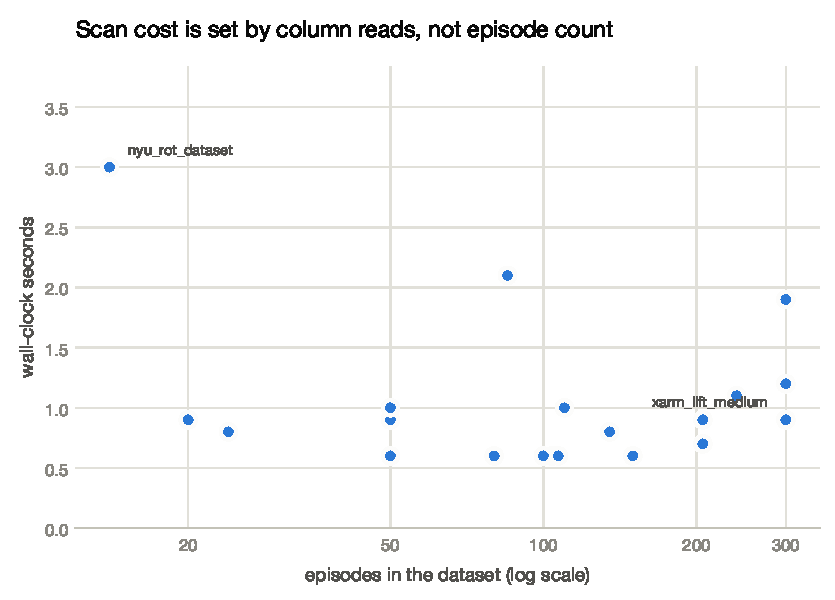
\includegraphics[width=0.82\textwidth]{../figures/fig3_runtime.pdf}
\caption{Scan wall-time against dataset size (log $x$). The relationship is flat: bohrin
reads Parquet columns and never decodes video, so per-dataset cost is dominated by fixed
per-detector work rather than by frame count.}
\label{fig:runtime}
\end{figure}

\begin{figure}[tb]
\centering
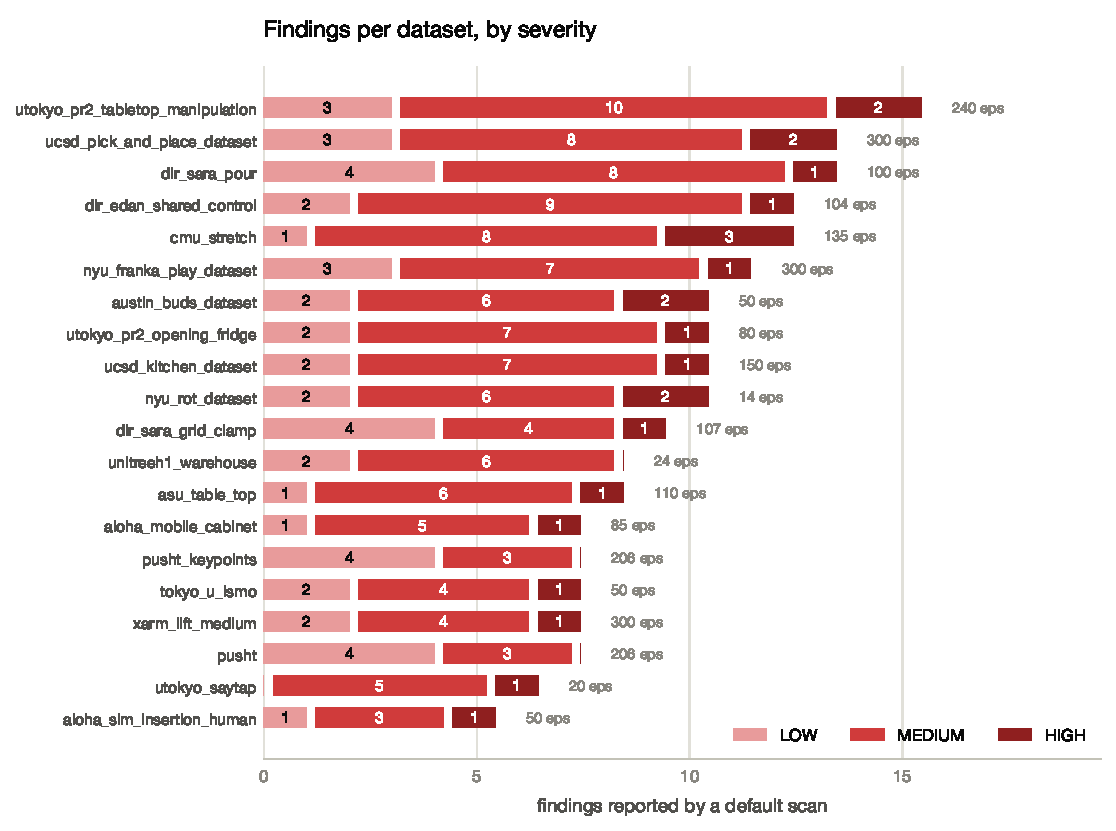
\includegraphics[width=0.88\textwidth]{../figures/fig2_dataset_severity.pdf}
\caption{Findings per dataset, split by severity. Every dataset produced findings; 17 of
20 produced at least one \textsc{high}.}
\label{fig:severity}
\end{figure}

\subsection{Precision measurement}

Of the 46 detectors that run in a default scan (48 registered, 2 held back; see
Section~\ref{sec:excluded}), \textbf{27 fired at least once} and \textbf{19 never fired on
any dataset}. Only \textbf{four} ever reached \textsc{high}
(Table~\ref{tab:high}, Figure~\ref{fig:rates}).

\begin{figure}[tb]
\centering
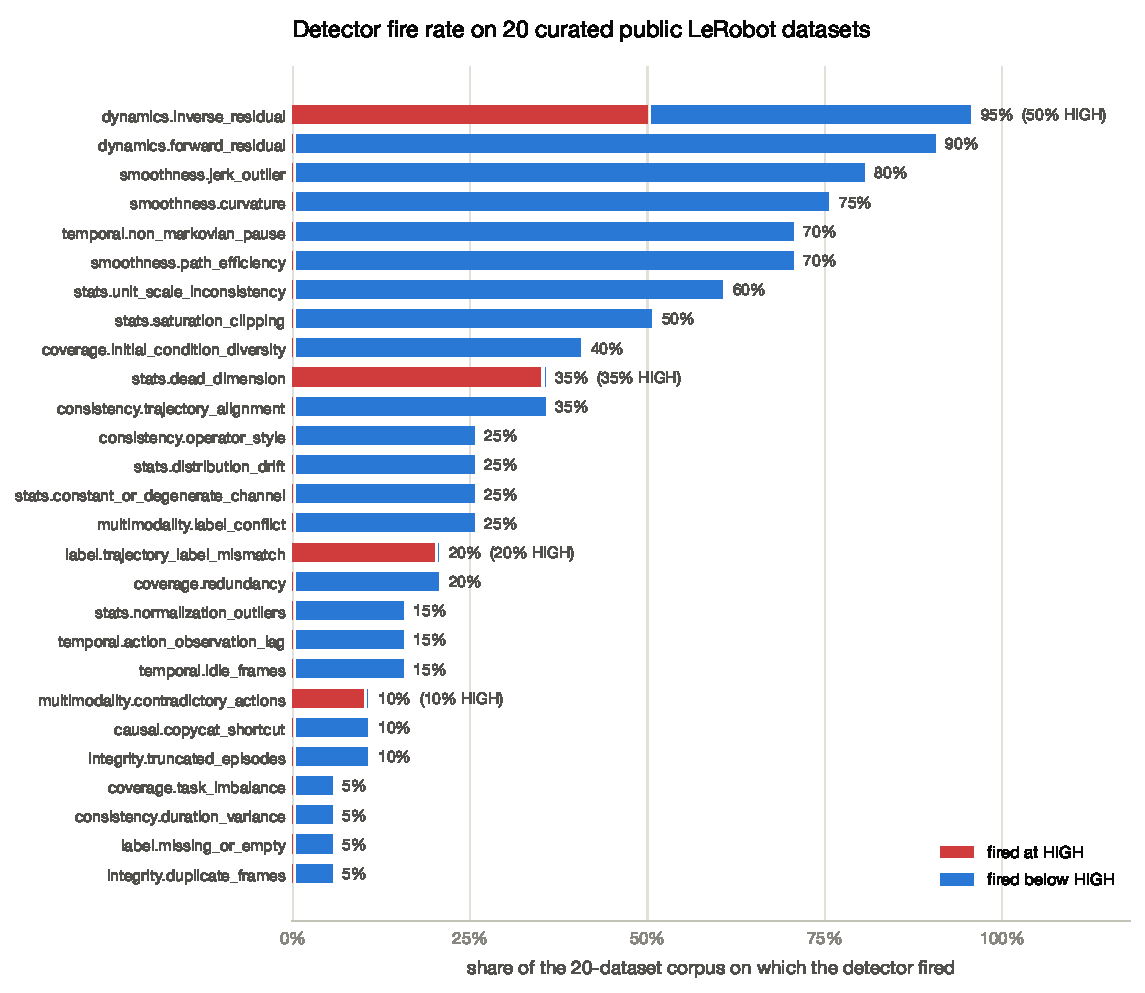
\includegraphics[width=0.90\textwidth]{../figures/fig1_detector_fire_rates.pdf}
\caption{Per-detector fire rate across the 20-dataset corpus, with the \textsc{high} share
called out in red. Twenty-seven detectors appear; the other nineteen produced no finding
on any dataset.}
\label{fig:rates}
\end{figure}

\begin{table}[tb]
\centering
\caption{The four detectors that ever reported \textsc{high}.}
\label{tab:high}
\small
\begin{tabular}{lrrl}
\toprule
Detector & Fires on & of which \textsc{high} & Reading \\
\midrule
\dtr{dynamics.inverse\_residual}        & 95\% & \warn{50\%} & Under suspicion (\S\ref{sec:suspect}) \\
\dtr{stats.dead\_dimension}             & 35\% & 35\% & Plausible; dead dims are common \\
\dtr{label.trajectory\_label\_mismatch} & 20\% & 20\% & Plausible at this rate \\
\dtr{multimodality.contradictory\_actions} & 10\% & 10\% & Plausible at this rate \\
\bottomrule
\end{tabular}
\end{table}

\subsection{\dtr{dynamics.inverse\_residual} is the outstanding problem}
\label{sec:suspect}

This detector fires on 19 of 20 datasets and returns \textsc{high} on 10 of 20. A detector
that reports \textsc{high} on half of a curated, published, widely used corpus is more
likely to have a threshold defect than to have found an epidemic.

Two readings are consistent with the number, and this sweep cannot distinguish them.
\emph{(i)~The threshold is loose:} the residual of a fitted inverse-dynamics model
$g(o_t, o_{t+1}) \rightarrow \hat{a}_t$ is compared against a bound that ordinary sensor
noise and 5\,Hz sub-sampling routinely exceed --- and most of this corpus is 5\,Hz, slow
enough that consecutive states are only weakly related by the logged action.
\emph{(ii)~The finding is real:} action/observation misalignment is a common defect in
converted datasets, and most of this corpus originates as RLDS/Open-X conversions rather
than native LeRobot recordings. Distinguishing these requires the adjudication described
in Section~\ref{sec:limits}.

\subsection{The nineteen silent detectors}

Nineteen of the 46 default detectors produced no finding across 2{,}631 episodes. This is
not evidence that they are broken --- several target defects this corpus should not have
(\dtr{integrity.nan\_inf}; the vision family, with decoding disabled; the entire
\textsc{policy}$\leftrightarrow$\textsc{data} family, which stays silent without a
checkpoint). It does mean those detectors carry \emph{zero real-data evidence} in this run,
and their default severities rest on synthetic fixtures alone. It would be incorrect to
describe this run as having validated 46 detectors.

\section{Two Detectors Were Correctly Held Back}
\label{sec:excluded}

Bohrin's registry defines \texttt{DEFAULT\_EXCLUDED}: detectors that are implemented,
tested, and benchmarked, but withheld from a default scan pending recalibration and
reachable with \texttt{-{}-all}. It currently holds \dtr{smoothness.discontinuity\_jump}
and \dtr{integrity.declared\_mismatch}, excluded after an earlier run of this same harness
measured them reporting \textsc{high} on 70\% and 60\% of the corpus respectively. Neither
appears in any finding in this sweep, confirming the mechanism works.

This is the project's stated alternative to deleting a noisy detector: measure it, record
the number, and gate it. Removing tested, benchmarked code to make a report look cleaner
is a regression, not a cleanup.

\section{Limitations}
\label{sec:limits}

These bound every number above and should be read before any of them is quoted.

\textbf{Fire rate is not precision.} Nothing here establishes that a single finding is
correct. A 95\% fire rate is equally consistent with ``95\% of public robot datasets have
this defect'' and with ``the threshold is too tight.'' No ground-truth labels exist for
this corpus and none were constructed. \emph{Every rate reported here is a rate of
complaint, not a rate of correctness.} The next step is to hand-adjudicate a stratified
sample against the underlying Parquet and publish a precision estimate with an explicit
$N$.

\textbf{Selection bias, in both directions.} The datasets were chosen by the project's own
maintainer. They are curated and widely used, which biases toward clean data and makes a
high fire rate \emph{more} suspicious --- the intended direction. But they are also
predominantly 5\,Hz Open-X/RLDS conversions, a narrow slice of how robot data is recorded,
so conversion-pipeline artifacts are over-represented.

\textbf{Single machine, single run.} One laptop (Apple M4, 16\,GB, macOS~15.5, Python
3.10.21), one pass, warm cache. Timings are indicative, not benchmarked: no repeats and no
confidence intervals.

\textbf{Default configuration only.} No checkpoint, target, calibration corpus, or vision.
The five \textsc{policy}$\leftrightarrow$\textsc{data} detectors were inert by
construction. A different configuration yields different numbers.

\textbf{The conformal gate was never active, and public metadata may prevent fixing that.}
Bohrin's \texttt{-{}-fpr} flag becomes a genuine false-discovery bound only when a
calibration corpus covers the dataset's embodiment --- Mondrian conformal prediction,
keyed on embodiment as the taxonomy. No corpus ships with the package, so every scan fell
back to a robust-$z$ heuristic. Filling that gap meets an obstacle this sweep surfaced
incidentally: \textbf{18 of the 20 datasets declare} \mbox{\texttt{robot\_type:\,"unknown"}}, with
only the two ALOHA datasets naming an embodiment. A Mondrian taxonomy keyed on a field
that 90\% of public data leaves blank collapses to a single wildcard bucket, forfeiting
exactly the group-conditional validity the design was chosen for. This is a finding about
ecosystem metadata hygiene as much as about the tool.

\textbf{Warnings observed, not investigated.} Several scans emitted
\mbox{\texttt{RuntimeWarning:\,divide by zero}} / \mbox{\texttt{overflow}} / \mbox{\texttt{invalid value}} from
\texttt{sklearn.utils.extmath} during dynamics fits. No scan failed and results are
reported as produced, but these indicate degenerate matrices reaching the ridge solve.

\section{Next Steps}

\begin{enumerate}\itemsep2pt
\item Adjudicate \dtr{dynamics.inverse\_residual} by hand-labelling a stratified sample of
its \textsc{high} findings. Either fix the threshold with the evidence, or add it to
\texttt{DEFAULT\_EXCLUDED} with the numbers recorded.
\item Publish a precision estimate with an explicit $N$. A measured number on 20
adjudicated findings is worth more than an unfalsifiable claim about 48 detectors.
\item Resolve the embodiment-metadata gap before shipping a default calibration corpus ---
either infer embodiment from action/state dimensionality and control rate, or accept the
wildcard bucket and stop claiming group-conditional validity.
\item Trace the \texttt{matmul} warnings in the dynamics fits.
\end{enumerate}

\section*{Reproducibility}

\begin{verbatim}
git clone https://github.com/prabhu-gopal/bohrin && cd bohrin
git checkout cf39d78
python -m venv .venv && .venv/bin/pip install -e '.[dev]'
.venv/bin/python scripts/hub_smoke.py --json sweep.json
\end{verbatim}

Raw results, figure-generation code, and this document's source are committed under
\path{benchmarks/2026-08-26-hub-sweep-v0.1.0/}. Every figure derives from
\texttt{results/sweep.json} alone; the committed JSON is the authority if a figure and the
text ever disagree. Hub dataset revisions are not pinned, so an upstream update will change
the numbers.

\vspace{0.6em}
\noindent\textcolor{ink}{\footnotesize Environment: Python 3.10.21, numpy 2.2.6,
polars 1.44.0, scikit-learn 1.7.2, huggingface-hub 1.28.0, pydantic 2.13.4, rich 15.0.0;
macOS 15.5 (Darwin 25.5.0), Apple M4, 16\,GB. Figures: matplotlib 3.11.1, generated in a
separate environment --- matplotlib is a reporting tool and deliberately not a bohrin
dependency.}

\end{document}
